\documentclass[12pt,a4paper]{scrartcl}

\usepackage[utf8]{inputenc}
\usepackage[T1]{fontenc}
\usepackage[british,UKenglish,USenglish,american]{babel}

\usepackage[pdftex]{graphicx}
\usepackage{latexsym}
\usepackage{amsmath,amssymb,amsthm}
\allowdisplaybreaks
\usepackage{dsfont}
\usepackage{pifont}
\usepackage{nicefrac}
\usepackage{textcomp}
\usepackage{enumitem}
\usepackage{lmodern}
\usepackage{bbm}

% Abstand obere Blattkante zur Kopfzeile ist 2.54cm - 15mm
\setlength{\topmargin}{-15mm}	   
                  
%\numberwithin{equation}{section} 
\numberwithin{equation}{subsection}

\newcommand{\C}{\mathbb{C}} % komplexe
\newcommand{\R}{\mathbb{R}} % reelle
\newcommand{\Q}{\mathbb{Q}} % rationale
\newcommand{\Z}{\mathbb{Z}} % ganze
\newcommand{\N}{\mathbb{N}} % natuerliche
\newcommand{\PP}{\mathbb{P}} % Probability
\newcommand{\E}{\mathcal{E}} % big Epsilon
\newcommand{\K}{\mathcal{K}}
\newcommand{\1}{\mathbbm{1}}
\newcommand{\G}{\mathcal{G}}
\newcommand{\GG}{\mathfrak{G}}

\numberwithin{equation}{section}

\theoremstyle{definition}
\newtheorem{example}{Example}[subsection]
\newtheorem{theorem}{Theorem}[subsection]
\newtheorem{corollary}{Corollary}[subsection]
\newtheorem{lemma}{Lemma}[subsection]
\newtheorem{definition}{Definition}[subsection]
\newtheorem{proposition}{Proposition}[subsection]
\newtheorem{algorithm}{Algorithm}[subsection]
\newtheorem{prop}{Proposition}[subsection]
\newtheorem{remark}{Remark}[subsection]
\newtheorem{pro}{Proof}
\newtheorem{comment}{Comment}[subsection]


\begin{document}
	\pagestyle{empty}

\begin{titlepage}

	
\includegraphics[scale=0.45]{kit-logo.jpg} 
    \vspace*{2cm} 
\begin{center} \large 
    
   Masterthesis
    \vspace*{2cm}

    {\huge External DLA}\\
    \vspace*{2.5cm}

    Tillmann Tristan Bosch
    \vspace*{1.5cm}

    10. March 2020
    \vspace*{3.5cm}


    Supervisor: PD. Dr. Steffen Winter \\[1cm]
    Faculty of Mathematics\\[1cm]
	Karlsruhe Institute of Technology
\end{center}
\end{titlepage}

\newpage

\newpage
\phantom \\
\newpage

\tableofcontents %Inhaltsverzeichnis

 	\pagestyle{headings}

\setcounter{page}{1}


\newpage

\section{Introduction}
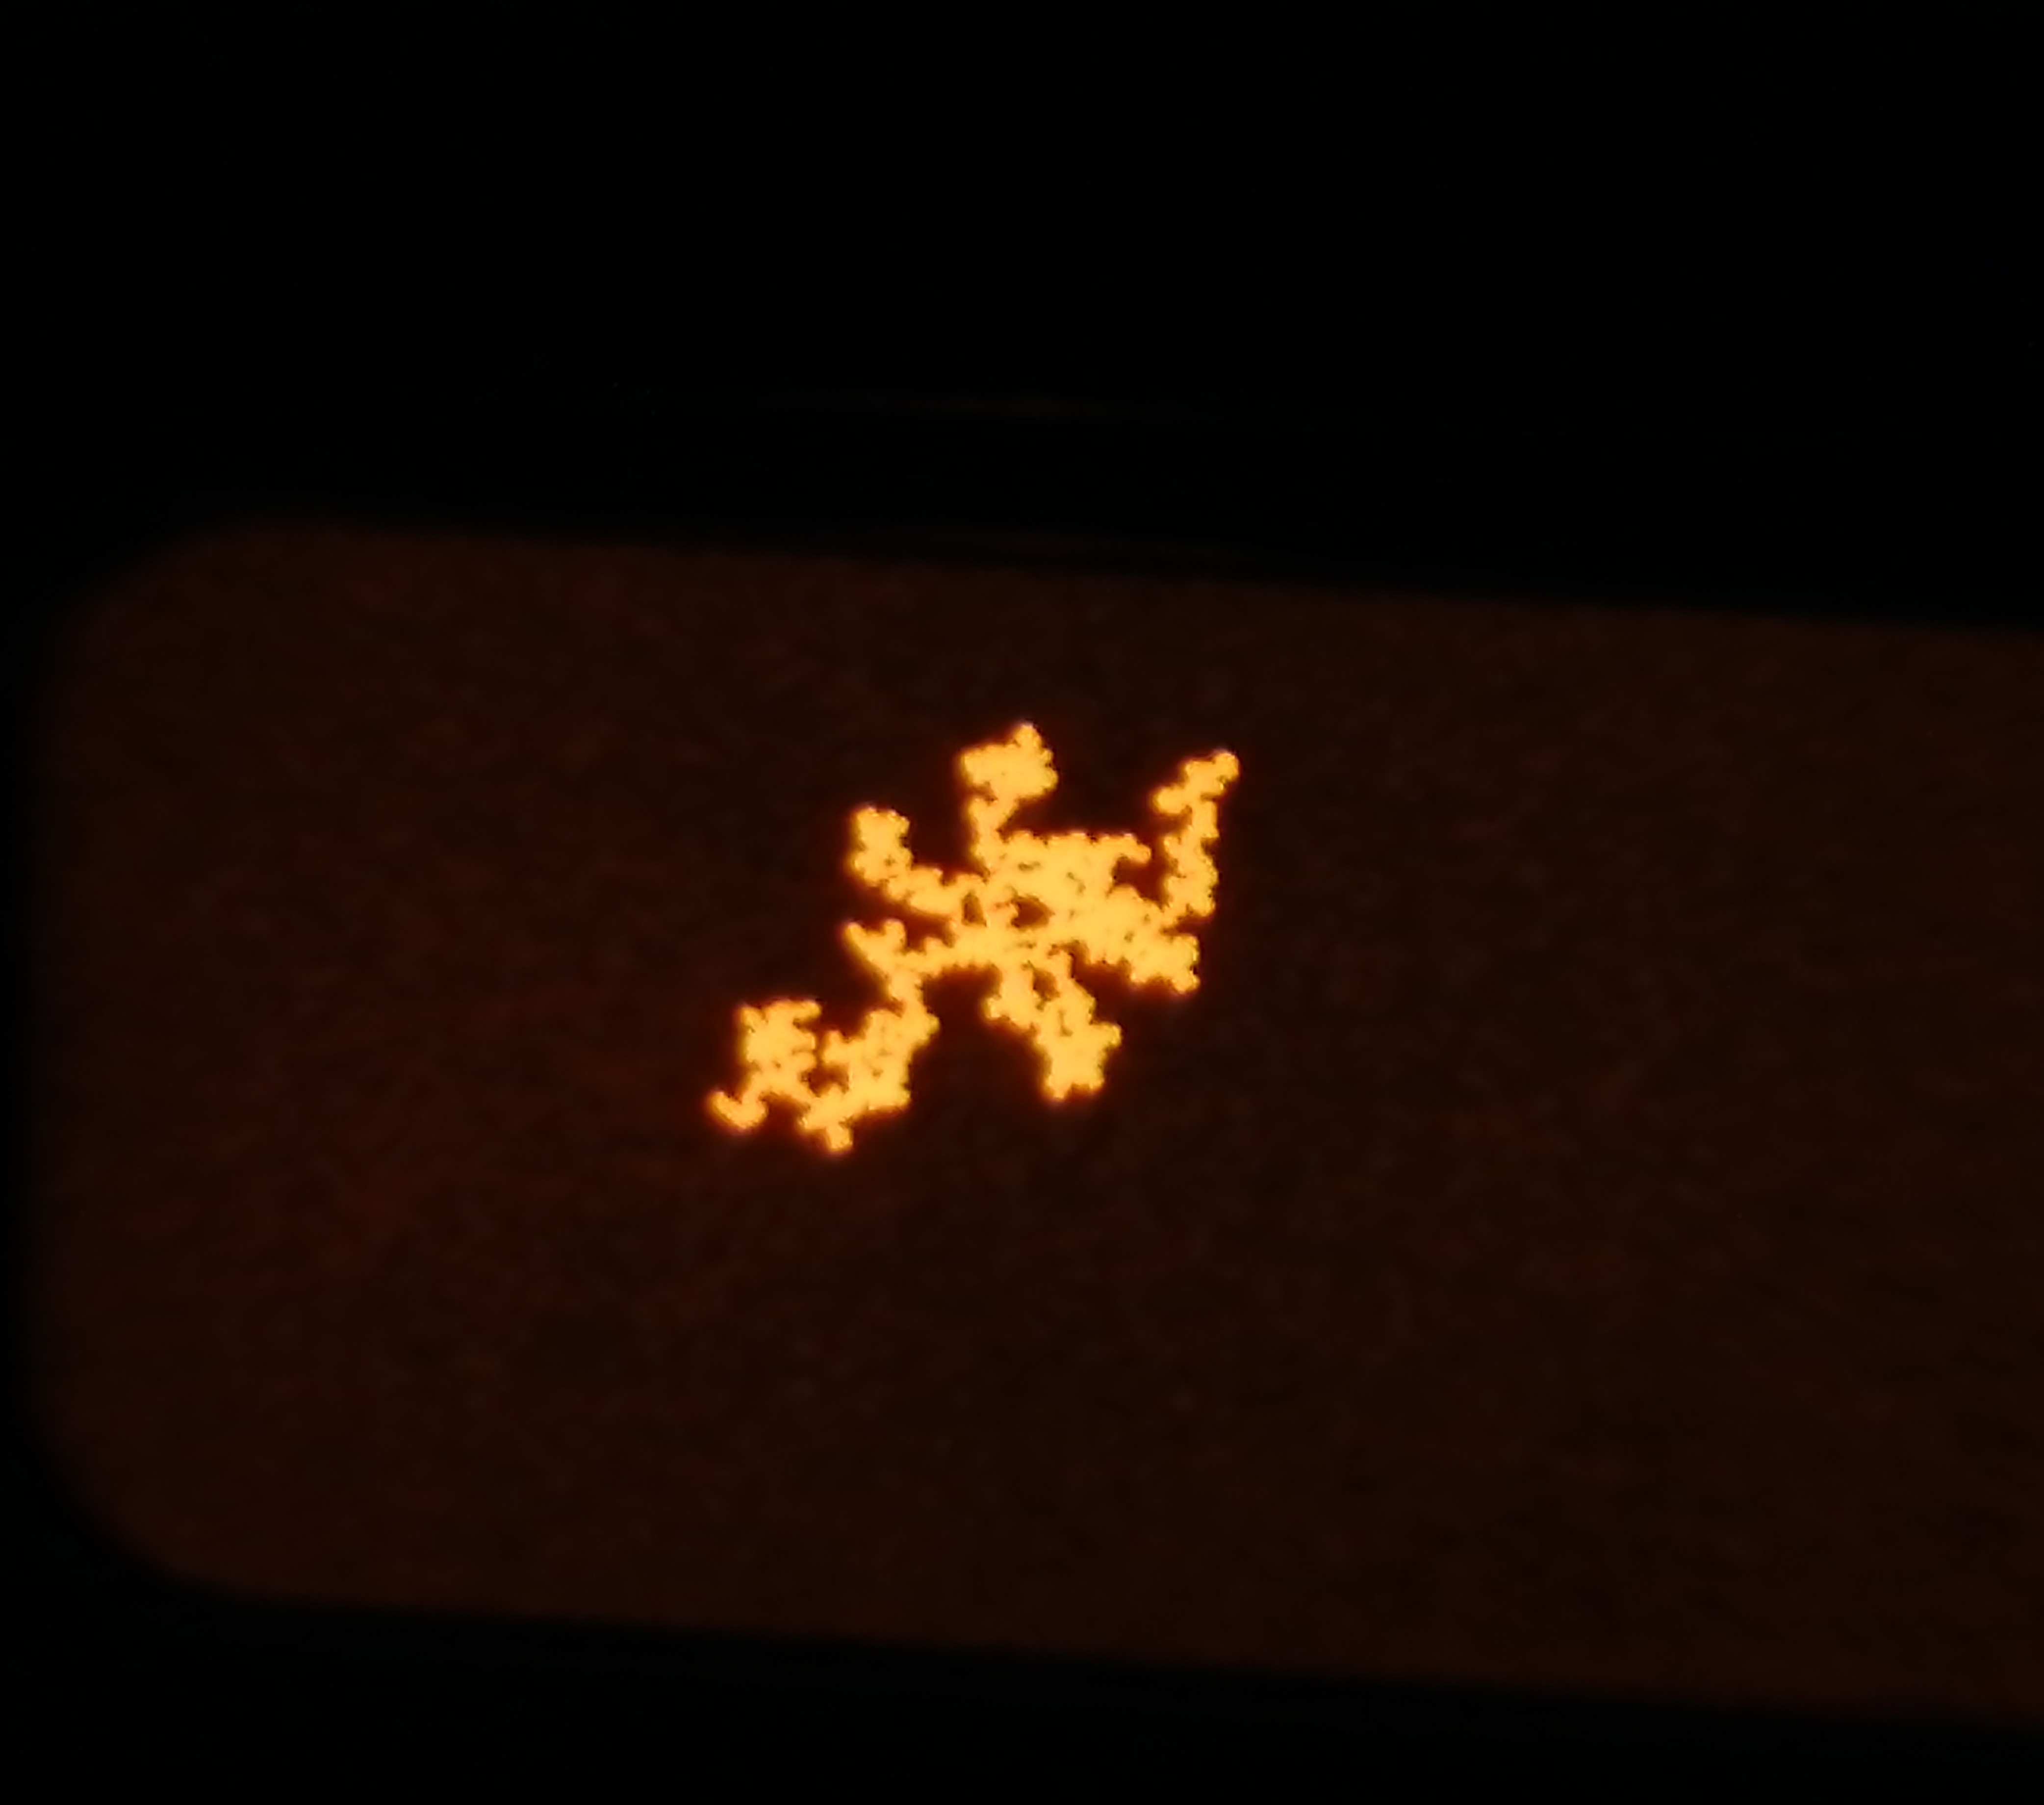
\includegraphics[scale=0.04]{display.jpg} 
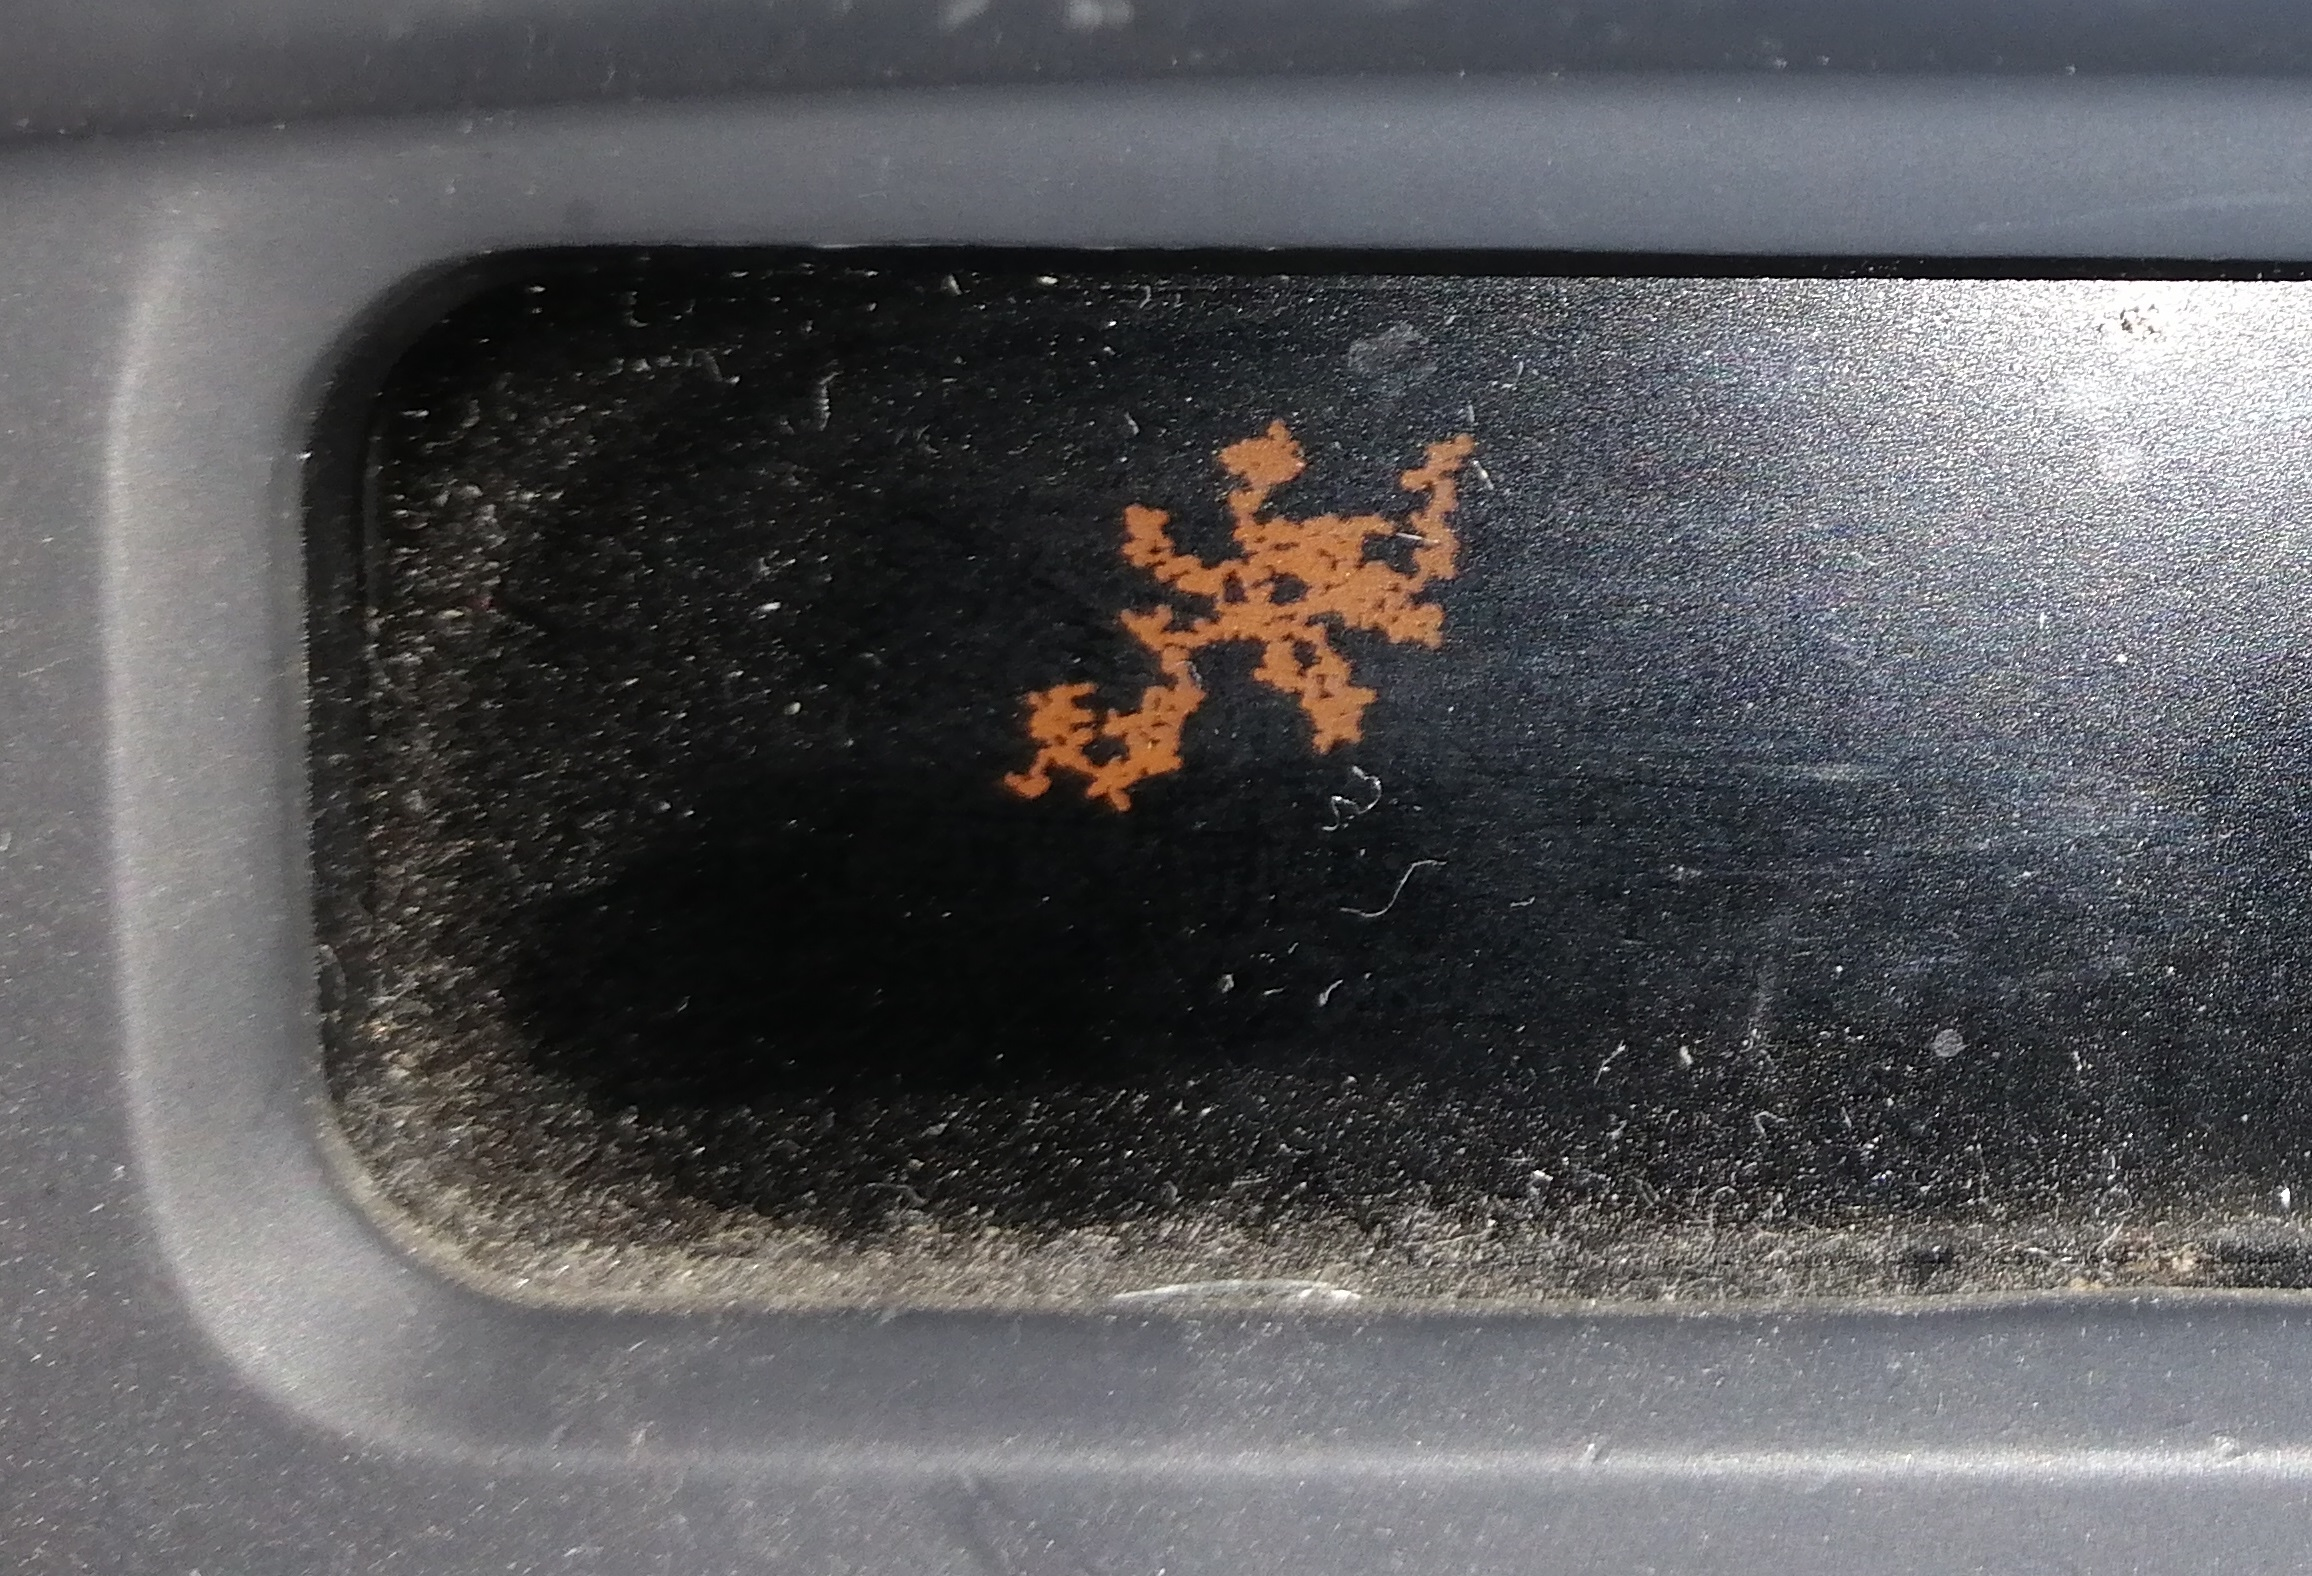
\includegraphics[scale=0.091]{display2.jpg}





\newpage


\section{Preliminaries} \label{prelim}

\subsection{Namings}
Here we list all namings which will be used in this paper. Let $d\in \N$ and $q\in \{0,\dots,d\}$. 
\begin{flalign*}
	&\N = \{1,2,3,\dots\} &&\text{set of natural numbers (without 0)}\\
	&\N_0 = \N\cup\{0\}\\
	&\K^d &&\text{set of convex and compact sets in }\R^d\\
	&B_d(r,x) = \{y\in \R^d\ |\ |x-y| \leq r\} &&\text{$d$-dimensional closed ball of radius $r$ around $x$}\\
	&S_{d-1}(r,x) = \partial B_d(r,x) &&\text{$(d-1)$-dimensional surface of the $d$-dimensional ball}\\
	&A(d,q) &&\text{set of q-dimensional affine subspaces of }\R^d \\
	&\mathcal{A}(d,q) &&\sigma\text{-algebra of } A(d,q), \text{ as constructed later in the paper} \\
	&\G := A(2,1) &&\text{set of lines in the real plane}\\
	&G_d &&\text{set of euclidean motions in $\R^d$ (rotations and translations)}
\end{flalign*}

\newpage
\subsection{Basic structures}

We prepare this script with the following preliminaries. Let $d\in \N$. \\

\noindent $\boldsymbol{\mathit{Graphs}}.\quad$ We will be interested in the graph $(\mathbb{Z}^d, E)$ with its canonical graph structure, which is two vertices (or points) $x=(x_1,\dots,x_d),y=(y.\text{real},\dots,y_d)\in \mathbb{Z}^d$ form an edge (e.q. $(x,y)\in E$) if and only if there exists exactly one $i\in \{1,\dots, d\}$ such that $|x_i - y_i| = 1$ and $x_j = y_j$ for all $j\neq i$. For a point $x\in \mathbb{Z}^d$ its set of $\mathit{neighbours}$ is defined as 
\begin{align*}
	N(x) := \{y\in \mathbb{Z}^d\ |\ (x,y)\in E\}.
\end{align*}
For a set $A\subset \mathbb{Z}^d$ the $\mathit{outer\ boundary}\ \partial A$ of $A$ is defined as 
\begin{align*}
	\partial A := \{y\in \mathbb{Z}^d\setminus A\ |\ \exists x\in A:\ (x,y)\in E\}
\end{align*}
Instead of $(\mathbb{Z}^d, E)$ we will write $\mathbb{Z}^d$ from now on. 
\\

\noindent $\boldsymbol{\mathit{Probability\ Space}}.\quad$ Let $(\Omega,\mathcal{F}, \mathbb{P})$ be a probability space which we will base on in this paper. For our space of interest $\mathbb{Z}^d$ we will always use the discrete $\sigma$-Algebra which is the power set of $\mathbb{Z}^d$. If for $A\in \mathcal{F}$ we have $\mathbb{P}(A)=1$ we will say that "$A$ holds $\mathbb{P}$-$a.s.$", or short "$A$ holds $a.s.$" (almost sure).
\\

\noindent $\boldsymbol{\mathit{Random\ Walk}}.\quad$ A family $(S_n)_{n\in \mathbb{N}}$ of measurable functions $S_n: \Omega \to \mathbb{Z}^d$ is called a $\mathit{Random\ Walk\ on}\ \mathbb{Z}^d$ $\mathit{(starting\ at}\ x\in \mathbb{Z}^d)$ if and only if $S_0=x$ $a.s.$ and $ S_n\in N(S_{n-1})$ $a.s.$ for all $n\geq 1$. It further shall hold that 

\begin{align*}
	\mathbb{P}(S_n = y) = \frac{1}{|N(S_{n-1})|} = \frac{1}{2d}\quad \text{ for all }  y\in N(S_{n-1})\quad a.s.
\end{align*}

\noindent Note that $|N(y)| = 2d$ for all $y\in \mathbb{Z}^d$ since every point has two neighbours in every dimension. So a Random Walk can be understood as a particle starting from some point $x$ and moving randomly on the grid choosing its next step uniformly from its neighbours. Further define 

\begin{align*}
	\mathbb{P}_x(S_n\in A) := \mathbb{P}(S_n\in A|S_0=x)
\end{align*}

\noindent for any subset $A\subset G$. We define the $hitting\ times$ of A 

\begin{align*}
	T_A := \min \{n\geq 0\ |\ S_n\in A\}\text{ and } T^+_A := \min \{n\geq 1\ |\ S_n\in A\}, 
\end{align*}

\noindent $T_x:= T_{\{x\}}$ and $T^+_x:= T^+_{\{x\}}$ for one element sets and $x\in \Z^d$. The $heat\ kernel$ of the random walk $S_n$ is defined to be 

\begin{align*}
	p_n(x,y):=\mathbb{P}_x(S_n=y)
\end{align*}

\noindent and the $\mathit{Green\ function}$ as 

\begin{align*}
	G(x,y) := \sum_{n\geq 0} p_n(x,y).
\end{align*}

$G$ is well-defined and finite since $\Z^2$ is transient. Similarily for a subset $A\subset G$ the $killed$ or $\mathit{stopped\ Green\ function}$ is defined as

\begin{align*}
	G_A(x,y) := \sum_{n\geq 0} \mathbb{P}_x(S_n=y, T_A > n).
\end{align*} 



\newpage
\section{Incremental Aggregate}
In this paper we will look at stochastic processes on the set of finite subsets of $\mathbb{Z}^d$, where we start with a one point set at $(0,0)$ and incrementally add a point on the outer boundary of the current cluster according to some distribution. What we get is a randomly, point-by-point growing connected cluster which here we will call $\mathit{Incremental\ Aggregate}$. Define 
\begin{align}
	\mathcal{P}_f := \{A\subset \mathbb{Z}^d\ |\ \text{A is finite}\}, 
\end{align}
the set of finite subsets of $\mathbb{Z}^d$. Furthermore we will be interested in distributions on those sets, so for $A\in \mathcal{P}_f$ we define 
\begin{align}
	\mathcal{D}_A:= \{\mu: \mathbb{Z}^d\to [0,1]\ |\ \mu(y) = 0 \text{ for all } y\notin A\ \text{and}\ \sum_{y\in A} \mu(y) = 1 \}, 
\end{align}
the set of distributions on $A$. Now we define $\mathit{Incremental\ Aggregate}$ as follows.  

\begin{definition}
	Let $\mu=(\mu_A)_{A\in \mathcal{P}_f}$ be a family of distributions with $\mu_A\in \mathcal{D}_A$ for all $A\in \mathcal{P}_f$. $\mathit{Incremental\ Aggregate\ (with\ distribution\ \mu)}$ is a stochastic process $(\mathcal{E}_n)_{n\in{\mathbb{N}_0}}$ which evolves as follows. The process starts with one point $\mathcal{E}_0 = \{(0,0)\}$ in the origin of $\mathbb{Z}^d$. Knowing the process $\mathcal{E}_n$ at time $n$, let $y_n$ be a random point in $\partial \mathcal{E}_n\in \mathcal{P}_f$ with distribution
	\begin{align}
		\mathbb{P}(y_n = y\ |\ \mathcal{E}_n) := \mu_{\partial \mathcal{E}_n}(y),\quad y\in \mathbb{Z}^d.
	\end{align}
	We then define $\mathcal{E}_{n+1} := \mathcal{E}_n \cup \{y_n\}$.
\end{definition} 

For all incremental aggregates in this paper we will have $d=2$, therefore move on the grid $\Z^2$. We will identify $\R^2$ with $\C$. 




\newpage

\newpage
\section{External DLA}

External DLA is a model of Incremental Aggregate as defined above using a very natural distribution, called the $\mathit{harmonic\ measure}$. 

\begin{definition} $\mathit{(Harmonic\ Measure)}$ Let $A\in\mathcal{P}_f$. Remembering the definitions in \eqref{prelim}, especially the heat kernel $p_n(x,y)=\mathbb{P}_x(S_n=y)$ of a random walk, for $x\in \Z^2$ the $\mathit{harmonic\ measure}$ (from $x$) of $A$ is
	\begin{align*}
	h_A(x,y) := \1\{y\in A\}p_{T_A}(x,y) = \1\{y\in A\}\PP_x(S_{T_A} = y),\quad \text{ for } y\in \Z^2.  
	\end{align*}
	We now define the $\mathit{harmonic\ measure}$ (from infinity) of $A$ as the family $h=(h_A)_{A\in \mathcal{P}_f}$ with
	\begin{flalign*}
		h_A(y) := \lim_{|x|\to\infty} h_A(x,y),\quad y\in \Z^2. 
	\end{flalign*}
	This is well-define because ... CONTINUE
\end{definition}

\begin{definition} $\mathit{(External\ Diffusion\ Limited\ Aggregate)}$ $\mathit{External\ Diffusion\ Limited\ Aggregate}$, short $\mathit{External\ DLA}$, is a incremental aggregate with the harmonic measure $h$ as distribution. 
\end{definition}



\newpage
\section{Integral Geometry}

In the next section we want to define an approximation for External DLA. This approximation will be a incremental aggregate for which definition of its distribution we need some concepts and results from Integral Geometry which we will discuss and develop in this section. The process we want to define bases on choosing a random line out of all lines which cut the current cluster of the aggregate. This random choosing is not obvious since the cluster most of times will be strongly not symmetric and it is even less obvious how to actually get a realisation of a random line when simulating with Python. In our case we are looking for a parametrisation of lines in the real plane and a reasonable way of choosing random parameters. \\

We will introduce a possible solution for this problem first through the abstract and general way of integral geometry and later through a simple parametrisation for the case of lines in the real plane which goes hand in hand with the general result.
 
\subsection{General results}

In the general context we are in $\R^d$ for $d\in \N$ and consider $q$-dimensional affine subspaces where $q\in \{0,\dots,d\}$, short $q$-flats in $\R^d$. The set of $q$-flats in $\R^d$ is denoted by $A(d,q)$. Later we will be interested in choosing random lines in the real plane (i.e. $1$-flats in $\R^2$). In order to get a probability measure on some set of $q$-flats, we first need a measure and a $\sigma$-algebra on $A(d,q)$ in total. 

\begin{definition}
	For $K\in \K^d$ define $A_K := \{F\in A(d,q)\ |\ F\cap K \neq\emptyset\}$. Then the $\sigma$-algebra $\mathcal{A}(d,q)$ on $A(d,q)$ shall be defined by
	\begin{flalign*}
		\mathcal{A}(d,q) := \sigma(\{ A_K\ |\ K\in \K^d\}).
	\end{flalign*} 
\end{definition}

After constructions which involve typical results in integral geometry like intrinsic volumes, Steiner Formula and the Crofton Formula we get the follwing theorem. Let $G_d = \{\varphi:\R^d \to\R^d,\ x\mapsto Ax+b\ |\ b\in R^d, A\in \R^{d\times d} \text{ with } A^TA=I\}$ be the set of euclidean motions in $\R^d$. 

\begin{theorem} \label{uniqmeas}
	On $A(d,q)$ there exists a unique $G_d$-invariant Radon measure $\mu_q$ such that
	\begin{flalign}
		\mu_q(A_{B_d(1,0)}) = \kappa_{d-q}, 
	\end{flalign}
	where $\kappa_n := \lambda_n(B_n(1,0))$ is the $n$-dimensional Lebesque meausure of the $n$-dimensional unit ball for $n\in \N$, and $\kappa_0:=1$.
\end{theorem}
\begin{proof}
	\cite{stoch1} Theorem 4.26
\end{proof}

\subsection{Construction in the real plane}

For our special case we choose $d=2$ and $q=1$, thus lines in the real plane, denoted by the set $\G$. The following construction is completely motivated by \cite{sackmann} 2.1.1. Firstly we propose a parametrisation of lines which works as following. Every line can be uniquely determined by an angle $\alpha\in [0,\pi)$ and a real number $p\in \R$. Let $e_\alpha := e^{\alpha i} = \cos(\alpha) + \sin(\alpha)i$ be the unit vector $1$ turned by $\alpha$ counterclockwise. It is easy to realize that $g_{\alpha,p} := \{x\in \C\ |\ \langle x,e_\alpha\rangle  = p\}$ defines a line and that every line has a unique pair of $\alpha$ and $p$ for such a representation. With $\Phi := [0,\pi) \times \R$ this naturally defines a bijection
\begin{flalign*}
	\chi: \Phi \to \G, \quad (\alpha,p) \mapsto g_{\alpha,p}. 
\end{flalign*}
We take the subspace Borel-$\sigma$-algebra $\mathcal{B}_\Phi:= \mathcal{B}^2 \cap \Phi$ on $\Phi$ and define the $\sigma$-algebra $\GG$ on $\G$ by $\GG := \chi(\mathcal{B}_\Phi)$. This works well since $\chi$ is a bijection. The next lemma shows that this way of defining a $\sigma$-algebra on $\G$ makes sense as it is indeed equivalent to the general context as defined above. 

\begin{lemma}
	We have $\GG=\mathcal{A}(2,1)$. 
\end{lemma}
\begin{proof}
	To proof this it is helpful to consider generators of these $\sigma$-algebras. Define the set of closed rectangles in $\Phi$ as $R := \{[a,b]\times[c,d]\subset \R^2\ |\ 0\leq a<b<\pi,c<d\}$. Then by measure theory we know that $\mathcal{B}_\Phi = \sigma (R)$ and since $\chi$ is a bijection, we have $\chi(\sigma (R)) = \sigma (\chi(R))$ and finally $\GG = \sigma(\chi(R))$. For $\tilde A := \{A_K\ |\ K\in \K^2\}$ we have by definition $\mathcal{A}(2,1) = \sigma(\tilde A)$. \\
	\indent $\subset$: CONTINUE
\end{proof}

\begin{definition}
	A $\mathcal{F}$-$\GG$-measurable function $g:\Omega \to \G$ is called a $\mathit{random\ line}$.  
\end{definition}

\begin{definition}
	We define the measure $\mu := {\lambda_2}_{|\Phi} \circ \chi^{-1}$ on $(\G,\GG)$ where ${\lambda_2}_{|\Phi}$ is the $2$-dimensional Lebesgue measure restricted to $\Phi$. We say a measure $\nu$ on $(\G,\GG)$ is locally finite if for any $K\in \K^2$ we have $\nu(A_K)<\infty$. 
\end{definition}

\begin{lemma}
	$\mu$ is locally finite and $G_2$-invariant. 
\end{lemma}
\begin{proof}
	Let $K\in \K^2$ and since $K$ is compact choose $r> 0$ such that $K\subset B_r$. Then we have $A_K\subset A_{B_r}$ and
	\begin{flalign*}
		\mu(A_K) \leq \mu(A_{B_r}) = {\lambda_2}_{|\Phi} (\chi^{-1}(A_{B_r})) = {\lambda_2}_{|\Phi}([0,\pi)\times [-r,r]) = 2\pi r < \infty, 
	\end{flalign*}
	hence $\mu$ is locally finite. CONTINUE 
\end{proof}

By \ref{uniqmeas} we know that $\mu$ is, up to a factor, the only euclidean motion invariant measure on $\G$. Since it is locally finite, for $K\in \K^2$ we can define a probability measure on $\G$ by
\begin{flalign*}
	\PP^K_\mu(A) := \frac{\mu( A\cap A_K)}{\mu(A_K)},\quad A\in \GG.
\end{flalign*}

\begin{definition}
	Let $K\in\K^2$. A random line $g:\Omega \to \G$ is called $K$-$\mathit{isotropic}$ if it is distributed as 
	\begin{flalign*}
		\PP(g\in A) = \PP^K_\mu(A),\quad A\in\GG.
	\end{flalign*}
\end{definition}

\begin{lemma}\label{circ}
	Let $M,K\in \K^2$ with $M\subset K$. Let $f$ be a random $K$-isotropic and $g$ be a random $M$-isotropic line. Then for all $A\in \GG$ we have
	\begin{flalign*}
		\PP(f\in A\ |\ f\in A_M) = \PP(g\in A).
	\end{flalign*}
\end{lemma}
\begin{proof}
	Note that since $M\subset K$ it is $A_M\subset A_K$. For $A\in \GG$ we therefore directly get 
	\begin{flalign*}
		\PP(f\in A\ |\ f\in A_M) &= \frac{\PP(f\in A\cap A_M)}{\PP(f\in A_M)}\\
		&= \frac{\mu(A\cap A_M\cap A_K)}{\mu(A_K)}\frac{\mu(A_K)}{\mu(A_M\cap A_K)}\\
		&=\frac{\mu(A\cap A_M)}{\mu(A_M)} \\
		&= \PP(g\in A).
	\end{flalign*}
\end{proof}

If we choose a simple convex set such as $K=B_r :=B_2(r,0)$ then choosing random $K$-isotropic lines becomes a very intuitive and easy realizable task as the following lemma shows.

\begin{lemma} \label{chi}
	Let $K=B_r\in\K^2$ and let $(\alpha,p)\sim\mathcal{U}(\tilde\Phi)$ with $\tilde \Phi:=[0,\pi)\times [-r,r]=\chi^{-1}(A_K)\subset \Phi$. Then $\chi(\alpha,p)$ is a random $K$-isotropic line. 
\end{lemma}
\begin{proof}
	For $A\in\GG$ we get 
	\begin{flalign*}
		\PP(\chi(\alpha,p)\in A) &= \PP((\alpha,p)\in \chi^{-1}(A)) = \frac{{\lambda_2}_{|\tilde\Phi}(\chi^{-1}(A\cap A_K))}{{\lambda_2}_{|\tilde\Phi}(\chi^{-1}(A_K))}\\
		&=\frac{{\lambda_2}_{|\Phi}(\chi^{-1}(A\cap A_K))}{{\lambda_2}_{|\Phi}(\chi^{-1}(A_K))} = \frac{\mu(A\cap A_K)}{\mu(A_K)}.
	\end{flalign*}
\end{proof}

Both lemmas \ref{circ} and \ref{chi} give a useful help for realizing $K$-isotropic lines for complicated sets $K$. Lemma \ref{circ} tells us that we if we are looking for a $K$-isotropic line, we can actually take a convex, compact set $B$ which contains $K$ and realize $B$-isotropic lines. If we realize such a line and it happens that it intersects $K$, we know that its distribution is equal to trying to realize $K$-isotropic lines directly. And how to realize $B$-isotropic lines? Lemma \ref{chi} tells us that if we choose $B=B_r$ a ball with a big enough radius such that it contains $K$, then realizing $B$-isotropic lines comes by choosing the line parameters $\alpha $ and $p$ uniformly in $[0,\pi)$ and $[-r,r]$. Finally we have a practicable process of choosing random $K$-isotropic lines, even if $K$ happens to be very asymmetric and complicated. This gives the base to define a new Incremental Aggregate in the next section which tries to approximize External DLA. 

\newpage

\section{Line Hitting Aggregate}

In the following we will look at a process which is the approach of a simple approximation of external DLA on $\mathbb{Z}^2$. The idea is to let particles move on straight lines coming from infinity and add to the cluster when hitting it. Obviously in most cases particles cannot move completely straight on $\mathbb{Z}^2$. Therefore we will consider points in $\mathbb{Z}^2$ as the centers of unit squares and let the particles move on straight lines in the full plane $\mathbb{R}^2$. We consider a line hitting a point in $\mathbb{Z}^2$ if and only if it intersects with its unit square as defined in the following. 

\begin{definition} \label{squares}
	Define 
	\begin{align}
		\C_{sq} := \{[k - \frac{1}{2}, k + \frac{1}{2}] + [l- \frac{1}{2}, l + \frac{1}{2}]i \subset \C\ |\ k,l \in \mathbb{Z}\}, 
	\end{align} 
	note that $\C = \bigcup_{s\in \C_{sq}} s$. The canonical function
	\begin{align}
	sq: \mathbb{Z}^2 \to \C_{sq},\quad (k,l)\to [k - \frac{1}{2}, k + \frac{1}{2}] + [l- \frac{1}{2}, l + \frac{1}{2}]i
	\end{align}
	is bijective and intuitively identifies points in $\mathbb{Z}^2$ with squares in $\C$ which is $p$ is the center of the square $sq(p)$ for all $p\in \mathbb{Z}^2$. In the following when using a point $p\in \mathbb{Z}^2$ it will reference the point in $\mathbb{Z}^2$ or the corresponding square in $\C$ respecting the context. This bijection also naturally defines a graph structure on $\C_{sq}$, which is two squares $s_1, s_2\in \C_{sq}$ form an edge if and only if $sq^{-1}(s_1)$ and $sq^{-1}(s_2)$ form an edge in $\mathbb{Z}^2$. 
	\noindent For the following context we say a line $g$ $hits$ a point $p\in \mathbb{Z}^2$ if and only if $g\ \cap\ sq(p) \neq \emptyset$. 
	
\end{definition}

BILD Linie durch squares "hitting"\\

\begin{definition}
	Let $g=g_{\alpha,p}\in \G$ and $A\in \mathcal{P}_f$. We define 
	
	\begin{align*}
		g\cap A := \{ p\in A\ |\ g \text{ hits } p\}
	\end{align*}
	
	which is the subset of all points in $A$ which are hit by $g$. For the following we suppose $g\cap A \neq \emptyset$. We will define a total ordered relation $\triangleleft$ on $g\cap A$ which shall be defined equivalently for all $g\in \G$ and $A\in\mathcal{P}_f$ with $g\cap A \neq\emptyset$. We choose two points $x,y\in g\cap A$ and devide the definition of the relation $\triangleleft$ into four cases, which are the line going from left-bottom to right-top, left-top to right-bottom, parallel to the $x$-axis and parallel to the $y$-axis. Denote the real part of $x$ with $x.$real and the imaginary one with $x.$imag. \\
	\\
	$\mathit{Case}\ 1:\quad g\ \text{ is parallel to the x-axis}\quad \Leftrightarrow\quad \alpha = \frac{\pi}{2}$
	\begin{align*}
	x \triangleleft y \quad :\Leftrightarrow \quad x.\text{real} < y.\text{imag}
	\end{align*}\\
	$\mathit{Case}\ 2:\quad g\ \text{ is parallel to the y-axis}\quad \Leftrightarrow\quad \alpha = 0$
	\begin{align*}
	x \triangleleft y \quad :\Leftrightarrow \quad x.\text{imag} < y.\text{imag}
	\end{align*}\\
	$\mathit{Case}\ 3:\quad g\ \text{ is going from left-bottom to right-top}\quad \Leftrightarrow\quad \alpha\in (\frac{\pi}{2},\pi)$
	\begin{align*}
	x \triangleleft y \quad :\Leftrightarrow \quad
		\begin{cases}
			x.\text{real} < y.\text{real}, & \text{ if } x.\text{real} \neq y.\text{real}, \\
			x.\text{imag} < y.\text{imag}, & \text{ if } x.\text{real} = y.\text{real}.
		\end{cases}
	\end{align*}\\
	$\mathit{Case}\ 4:\quad g\ \text{ is going from left-top to right-bottom}\quad \Leftrightarrow\quad \alpha\in (0,\frac{\pi}{2})$
	\begin{align*}
	x \triangleleft y \quad :\Leftrightarrow \quad
	\begin{cases}
	x.\text{real} < y.\text{real}, & \text{ if } x.\text{real} \neq y.\text{real}, \\
	x.\text{imag} > y.\text{imag}, & \text{ if } x.\text{real} = y.\text{real}.
	\end{cases}
	\end{align*}\\
	It is easy to see that this well-defines a relation on $g\cap A$. In the following we will quickly proove that this relation is totally ordered. 
\end{definition}

\begin{lemma}
For a line $g=g_{\alpha,p}\in\G$ and $A\in \mathcal{P}_f$ with $g\cap A\neq \emptyset$ the relation $\triangleleft$ on $g\cap A$ is totally ordered. 
	\begin{proof}
		We will only proove the case where $g$ is going from left-bottom to right-top, which is $\mathit{Case}\ 3$ of the definition. In this case we have $\alpha\in (\frac{\pi}{2},\pi)$. Note, that the proof for $\mathit{Case\ }4$ will work very similair and in the case of $g$ being parallel to one of the axes ($\mathit{Case\ }1$ or $2$), all properties for a totally ordered relation follow directly from the totally ordered relation $<$ on $\mathbb{R}$. So let $\alpha\in (\frac{\pi}{2},\pi)$. \\
		\\
		$\mathit{Antisymmetry:}$ For antisymmetry let $x \triangleleft y$ and $y \triangleleft x$. Suppose $x.\text{real}\neq y.\text{real}$, then $x.\text{real} < y.\text{real}$ and $y.\text{real} < x.\text{real}$, therefore $x.\text{real} = y.\text{real}$ by antisymmetry of the standard order $<$ in $\mathbb{R}$, a contradiction, hence $x.\text{real} = y.\text{real}$. But then we have $x.\text{imag} < y.\text{imag}$ and $y.\text{imag} < x.\text{imag}$ and therefore also $x.\text{imag} = y.\text{imag}$. \\
		\\
		$\mathit{Transitivity:}$ For transitivity let $x \triangleleft y$ and $y \triangleleft z$. We find four cases. In case $x.\text{real} \neq y.\text{real}$ and $y.\text{real} \neq z.\text{real}$ we get $x.\text{real} < z.\text{real}$ by transitivity of $<$, hence $x \triangleleft z$. In case $x.\text{real}\neq y.\text{real}$ and $y.\text{real} = z.\text{real}$ we get $x.\text{real} < y.\text{real} = z.\text{real}$, therefore $x \triangleleft z$. In case $x.\text{real} = y.\text{real}$ and $y.\text{real} \neq z.\text{real}$ we get $x.\text{real} = y.\text{real} < z.\text{real}$, similair as the last case. In the last case $x.\text{real} = y.\text{real} = z.\text{real}$ we get $x.\text{imag} < y.\text{imag}$ and $y.\text{imag} < z.\text{imag}$ and again by transitivity of $<$ we get $x.\text{imag} < z.\text{imag}$, hence $x \triangleleft z$ again. \\
		\\
		$\mathit{Connexity:}$ Connexity is given since for any two points $x,y\in g\cap A$ we have either $x.\text{real} \neq y.\text{real}$ or $x.\text{real} = y.\text{real}$ and therefore either $x\triangleleft y$ or $y\triangleleft x$.
	 
	\end{proof}
\end{lemma}

\begin{remark}
	The relation $\triangleleft$ on $g\cap A$ basically orders the hitpoints of $g$ with $A$ from left to right (or bottom to top in case of a line parallel to the $y$-axis). This order allows us to identify the outest hitting points which are minimum and maximum of $g\cap A$ respecting $\triangleleft$. To clarify, we define $min (g\cap A) := x_0$ if and only if $x_0 \triangleleft x$ for all $x\in g\cap A$, analogously $max(g\cap A)$. This means when moving on $g$ facing $A$ coming from infinity this order allows to know where in $A$ the line $g$ hits first when "entering" $A$ and where it hits last when "leaving" $A$. 
\end{remark}

Remind, for a bounded subset $A\subset \C$ the convex hull $conv(A)$ of $A$ is defined to be the smallest convex set containing $A$, formally 
\begin{flalign*}
	conv(A) := \bigcap_{A\subset K\in \K^2} K. 
\end{flalign*}
Note that $conv(A)\in \K^2$ for all bounded subsets $A\subset \C$. For a set $A\in \mathcal{P}_f$ we define 
\begin{flalign*}
	conv(A):=conv(\bigcup_{p\in A} sq(p))
\end{flalign*}
and since $\bigcup_{p\in A} sq(p)$ is a bounded set we have $conv(A)\in \K^2$ here aswell. 

\begin{definition} $\mathit{(Random\ Line\ Hitting\ Distribution)}$ Let $A\in \mathcal{P}_f$ and $g:\Omega \to \G$ be a random $conv(A)$-isotropic line. Then define a distribution $\mu_A \sim \mathcal{U}(\{min(g\cap A), max(g\cap A)\})$, which chooses uniformly out of the outest hitting points of $g$ with $A$. We call this family $(\mu_A)_{A\in \mathcal{P}_f}$ of distributions the $\mathit{Random\ Line\ Hitting\ Distribution}$.
\end{definition}

\begin{definition} $(\mathit{Line\ Hitting\ Aggregate)}$ An Incremental Aggregate with the Random Line Hitting Distribution we call $\mathit{Line\ Hitting\ Aggregate}$, short $\mathit{LHA}$. 
\end{definition}

\newpage
\section{Python Simulation}
Part of the work in this paper is the attempt to build simulations for both incremental aggregates $\mathit{External\ DLA}$ and $\mathit{LHI}$ which were presented in the previous sections. For calculating the simulations we use $\mathit{Python}$ and for rendering pictures we use the package $\mathit{Pygame}$. Each vertex in $\Z^2$ is naturally mapped to its coordinate and is represented in this way in python code. In graphics each coordinate basically can be represented by squares in $\C$ as presented in Definition $\ref{squares}$, and each square will be represented by exactly one pixel, so every picture about incremental aggregates you'll see in the following consists of pixels each representing exactly one vertex in $\Z^2$ in the most natural way. Our aim will be to simulate the aggregates as close as possible to their mathematical definitions. This is much easier for LHI, and less obvious for External DLA. We start of with External DLA in the following.

\subsection{External DLA Simulation}

By identifying each vertex in $\Z^2$ with its square in $\C$ and a pixel when rendering, the representation of the space we are moving is exact. For any simulation of randomness we use the package $\mathit{random}$. Respecting the error behaviour of this package, random walks on $\Z^2$ can be simulated directly and therefore very exact. For External DLA we let a particle move randomly on the grid and wait for it to hit the actual cluster. The problem which will have to be solved is where to start the moving particle and how to handle a particle when it is moving away from the actual cluster, therefore creating a too long waiting time for it coming back to the cluster. In the definition of External DLA new particles start the random walk from infinity. Obviously this is not possible in simulation so this has to be solved differently. 



\subsection{LHI Simulation}



\newpage
\section{Questions}

\newpage

\begin{thebibliography}{biblio}
\thispagestyle{empty}

\bibitem{Henze Skript}
N. Henze.
\emph{Maß und Wahrscheinlichkeitstheorie (Stochastik II)}.
Karlsruher Institut für Technologie, Karlsruhe, 2010

\bibitem{stoch1}
Daniel Hug, Günter Last, Steffen Winter.
\emph{Stochastic Geometry, 	Lecture Notes (summer term 2020)}.
Institute of Technology, Karlsruhe, 2020

\bibitem{sackmann}
Franz Sackmann. 
\emph{Zufällige Geraden, Staatsexamensarbeit}.
University Karlsruhe (TH), Karlsruhe, 2007



\end{thebibliography}

\newpage
  
\thispagestyle{empty}

\vspace*{8cm}


\section*{Erklärung}

Hiermit versichere ich, dass ich diese Arbeit selbständig verfasst und keine anderen als die angegebenen Quellen und Hilfsmittel benutzt, die wörtlich oder inhaltlich übernommenen Stellen als solche kenntlich gemacht und die Satzung des Karlsruher Instituts für Technologie zur Sicherung guter wissenschaftlicher Praxis in der jeweils gültigen Fassung beachtet habe. \\[2ex] 

\noindent
Karlsruhe, den 10. März 2020\\[5ex] 

\end{document}

